% ----------------------------------------------------------------------------------------
% Sta Maria 2013
%
% Nelson Lu�s Dias --
% 2013-11-19T17:06:20
% ----------------------------------------------------------------------------------------
\documentclass[20pt,Screen4to3,headrule,footrule]{foils}
\usepackage[headsep=3ex,hscale=0.9,rmargin=1.75cm,lmargin=1.75cm,tmargin=2.5cm,bmargin=2cm]{geometry}
\usepackage[T1]{fontenc}                          
\usepackage[brazil]{babel}
\usepackage{amsmath}
\usepackage{amssymb}
\usepackage{textcomp}
\usepackage{stmaryrd}
%\usepackage{bm}
% 
% package relsize: needed only if you use \mathlarger, \mathsmaller!!!
%\usepackage{relsize}
%
\def\Xint#1{\mathchoice
{\XXint\displaystyle\textstyle{#1}}%
{\XXint\textstyle\scriptstyle{#1}}%
{\XXint\scriptstyle\scriptscriptstyle{#1}}%
{\XXint\scriptscriptstyle\scriptscriptstyle{#1}}%
\!\int}
\def\XXint#1#2#3{{\setbox0=\hbox{$#1{#2#3}{\int}$}
\vcenter{\hbox{$#2#3$}}\kern-.5\wd0}}
\def\ddashint{\Xint=}
\def\dashint{\Xint-}

% ---------------------------------------------------------------------------
% use Euler Fonts for my own devious ends
% ---------------------------------------------------------------------------
\DeclareMathAlphabet\EuScript{U}{eus}{m}{n}
\SetMathAlphabet\EuScript{bold}{U}{eus}{b}{n}


\newcommand{\bbxfamily}{\fontencoding{U}\fontfamily{bbold}\selectfont}
\newcommand{\textbbx}[1]{{\bbxfamily#1}}
\DeclareMathAlphabet{\mathbbx}{U}{bbold}{m}{n}
\DeclareMathAlphabet{\mathpzc}{OT1}{pzc}{m}{it}
\newcommand{\zapf}{\fontencoding{OT1}\fontfamily{pzc}\fontseries{m}\fontshape{it}\fontsize{16}{16pt}\selectfont}
% ---------------------------------------------------------------------------
% math.tex was originally developed as a set of TeX macros.  Here, it
% is being modified for LaTeX use, so you wil find a mix of TeX and
% LaTeX commands (sorry...).  At any rate, it provides some useful
% macros.  Take a look
%
% Nelson Lu\'{\i}s Dias
% 15 apr 1994
% 27 sep 1996
% 27 sep 2002
% ---------------------------------------------------------------------------
%\newcounter{ItemNumber} %
% ---------------------------------------------------------------------------
% the fourier-transform of long expressions is typed as a wide hat after
% the expression
% ---------------------------------------------------------------------------
\newcommand{\aft}{\widehat{\phantom{u}}}
% ---------------------------------------------------------------------------
% macros to simplify math typing
% ---------------------------------------------------------------------------
\DeclareMathOperator{\sen}{sen}%
\DeclareMathOperator{\senh}{senh}%
\DeclareMathOperator{\tg}{tg}%
\DeclareMathOperator{\tgh}{tgh}%
\DeclareMathOperator{\cotgh}{cotgh}%
\DeclareMathOperator{\snl}{snl}
\DeclareMathOperator{\arcsen}{arcsen}%
\DeclareMathOperator{\erf}{erf}%
\DeclareMathOperator{\erfc}{erfc}%
\DeclareMathOperator{\haversin}{haversin}%
\DeclareMathOperator{\arcsenh}{arcsenh}%
\DeclareMathOperator{\arctg}{arctg}%
\DeclareMathOperator{\arctgyx}{arctg2}%
\DeclareMathOperator{\cis}{cis}%
\newcommand{\arctgh}{{\rm arctgh}}%
\newcommand{\blob}{\; \mbox{\rule{4pt}{4pt}}}%
\newcommand{\bfvec}[1]{\mathord{\mbox{\bf #1}}}%
\newcommand{\cotg}{{\rm cotg\,}}%
\newcommand{\cross}{\vet{\times}}
\newcommand{\deriva}[2]{\frac{d{#1}}{d{#2}}}%
\newcommand{\mderiva}[2]{\frac{\md{#1}}{\md{#2}}}%
\def\dbar{{\raisebox{-0.75pt}{$\mathchar'26$}\mkern-14.5mu\mathrm{d}}} 
\newcommand{\dimof}[1]{\left\llbracket #1 \right\rrbracket}
\DeclareMathOperator{\Cov}{Cov}%
\DeclareMathOperator{\Var}{Var}%
\DeclareMathOperator{\MSE}{MSE}
\DeclareMathOperator{\RMSE}{RMSE}
\DeclareMathOperator{\EMQ}{EMQ}%
\DeclareMathOperator{\REMQ}{REMQ}
\DeclareMathOperator{\Exv}{E}%
\DeclareMathOperator{\Co}{Co}
\DeclareMathOperator{\Qu}{Qu}
\DeclareMathOperator{\Rea}{Re}
\DeclareMathOperator{\Img}{Im}
% ----------------------------------------------------------------------------
% \derder must be considered obsolete, but is kept for backward compatibility;
% \dern is preferable
% ----------------------------------------------------------------------------
\newcommand{\derder}[3]{%
   \frac{d^{#3}{#1}}
        {d{#2}^{#3}}
}%
\newcommand{\dern}[3]{%
   \frac{d^{#3}{#1}}
        {d{#2}^{#3}}
}%
\newcommand{\mdern}[3]{%
   \frac{\md^{#3}{#1}}
        {\md{#2}^{#3}}
}%
\newcommand{\dmat}[1]{\frac{ D{#1}}{Dt}}%
\newcommand{\dmatbar}[1]{\frac{ \overline{D}{#1}}{Dt}}%
\newcommand{\fof}[1]{\mathord{\mbox{\large\it ff}\,{(#1)}}}%
\newcommand{\ifonlyif}{{\; \Leftrightarrow \;}}%
\providecommand{\implies}{\; \Rightarrow \;}%
\newcommand{\then}{\; \Rightarrow \;}%
\newcommand{\parder}[2]{ {\frac{\partial {#1}}{\partial{#2}} }}%
\newcommand{\thermopar}[3]{{\left(\frac{\partial {#1}}{\partial{#2}}\right)_{#3} }}%

\newcommand{\parpar}[3]{\frac{\partial^2 {#1}}{\partial{#2} \partial{#3}}}%
\newcommand{\parparpar}[4]{\frac{\partial^3 {#1}}{\partial{#2} \partial{#3}\partial{#4}}}%
\newcommand{\parn}[3]{%
    \frac{\partial^{#3} {#1}}%
         {\partial {#2}^{#3}}
}%
\newcommand{\parpow}[2]{ {\left( #1 \right) }^{#2} }%
\newcommand{\such}{\;|\;}%
\newcommand{\totder}[2]{ {D{#1} \over D{#2} } }%
\newcommand{\ulvec}[1]{\underline{#1}}
%\def\well#1{\mathstrut #1}%
%\def\I{\, \mathord{\sl i}\, }%
% ---------------------------------------------------------
% the classic sets
% ---------------------------------------------------------
\newcommand{\rea}{\mathbb{R}}%
\newcommand{\com}{\mathbb{C}}%
\newcommand{\reb}{\mathbb{R}^2}%
\newcommand{\ren}{\mathbb{R}^n}
% ---------------------------------------------------------
% math formulas, displaystyle, in LR mode
% ---------------------------------------------------------
\newcommand{\mathbox}[1]{%
\mbox{$\displaystyle #1$}%
}
\newcommand{\tavg}[1]{\left\langle #1 \right\rangle}
\newcommand{\tavh}[1]{\langle #1 \rangle}
% -----------------------------------------------------------------------------
% e e i
% -----------------------------------------------------------------------------
\newcommand{\me}{\mathrm{e}}
\newcommand{\mi}{\mathrm{i}}
\newcommand{\md}{\mathrm{d}}
%% \newcommand{\md}{\mathord{\textsl{d}}}
%% \newcommand{\mi}{\mathord{\textsl{i}}\,}
%% \newcommand{\me}{\mathord{\textsl{e}}}

% ---------------------------------------------------------------
% minha redefini��o local de vetor
% ---------------------------------------------------------------
%\newcommand{\vet}[1]{\mathbf{#1}}
\newcommand{\bdot}{\boldsymbol{\cdot}}
\newcommand{\vet}[1]{\boldsymbol{#1}}
\newcommand{\vut}[1]{\ensuremath{\mathbf{#1}}}
\newcommand{\vem}[1]{\underset{\sim}{#1}}
\newcommand{\ven}[1]{\underset{\approx}{#1}}
\newcommand{\veg}[1]{\mathord{\mbox{\boldmath $#1$}}}
%\newcommand{\mat}[1]{\mathord{[\mbox{\boldmath $#1$}]}}
%\newcommand{\met}[1]{\mathord{\mbox{\boldmath $[#1]$}}}
\newcommand{\met}[1]{\mbox{$\boldsymbol{[}$} \boldsymbol{#1} \mbox{$\boldsymbol{]}$}}
\newcommand{\mat}[1]{\mbox{$\boldsymbol{[}$} #1 \mbox{$\boldsymbol{]}$}}
\newcommand{\mut}[1]{\ensuremath{\mathbf{[#1]}}}
% --------------------------------------------------------------------
% mathptmx requires a special treatment
% --------------------------------------------------------------------
%\newcommand{\mut}[1]{\mathord{\mbox{       $\bm{[#1]}$}}}
% --------------------------------------------------------------------
% 
% --------------------------------------------------------------------
\newcommand{\bigmat}[1]{\mbox{$\boldsymbol{\big[}$} #1 \mbox{$\boldsymbol{\big]}$}}
\newcommand{\Bigmat}[1]{\mbox{$\boldsymbol{\Big[}$} #1 \mbox{$\boldsymbol{\Big]}$}}
\newcommand{\biggmat}[1]{\mbox{$\boldsymbol{\bigg[}$} #1 \mbox{$\boldsymbol{\bigg]}$}}
\newcommand{\Biggmat}[1]{\mbox{$\boldsymbol{\Bigg[}$} #1 \mbox{$\boldsymbol{\Bigg]}$}}
\newcommand{\ten}[1]{\mathbb{#1}}
\newcommand{\mlin}[1]{[#1]^{\mathsf{\small T}}}
%\newcommand{\tr} {{\mbox{\tiny$\mathsf{T}$}}}
\newcommand{\tr} {{\mbox{\tiny$\boldsymbol{\top}$}}}
\newcommand{\adj}{{\mbox{\tiny$\dagger$}}}
\newcommand{\tuplet}[1]{({#1}_1,{#1}_2,{#1}_3)}
\newcommand{\tuplen}[1]{({#1}_1,{#1}_2,\ldots,{#1}_n)}
\newcommand{\jac}[2]{\frac{\partial\tuplen{#1}}{\partial\tuplen{#2}}}
% -----------------------------------------------------------------------------
% latitude, longitude
% -----------------------------------------------------------------------------
\newcommand{\latmin}[3]{#1\textdegree\,#2\textquotesingle\,#3}
\newcommand{\lonmin}[3]{#1\textdegree\,#2\textquotesingle\,#3}
% -----------------------------------------------------------------------------
% � fun��o de/ n�o � fun��o de
% -----------------------------------------------------------------------------
%\newcommand{\isfunc}[1]{\mbox{=\textflorin}(#1)}
\newcommand{\isfunc}[1]{:=\text{f{\kern-0.1em}f}(#1)}
\newcommand{\isnotfunc}[1]{:\ne\text{f{\kern-0.1em}f}(#1)}
\newcommand{\isconst}[1]{:=\text{\textcent}}
\newcommand{\inner}[2]{\langle {#1},{#2} \rangle}
% ---------------------------------------------------------------------------
% macros to produce uppercase greek letters
% ---------------------------------------------------------------------------
\newcommand{\Alpha}{\mathord{\mathcal{A}}}
\newcommand{\Beta}{\mathord{\mathcal{B}}}
\newcommand{\Epsilon}{\mathord{\mathscr{E}}}
\newcommand{\Zeta}{\mathord{\mathcal{Z}}}
\newcommand{\Eta}{\mathord{\mathcal{H}}}
\newcommand{\Iota}{\mathord{\mathcal{I}}}
\newcommand{\Kappa}{\mathord{\mathcal{K}}}
\newcommand{\Mu}{\mathord{\mathcal{M}}}
\newcommand{\Nu}{\mathord{\mathcal{N}}}
% \newcommand{\omicron}{\mathord{o}}
\newcommand{\Omicron}{\mathord{\mathcal{O}}}
%\newcommand{\Rho}{\mathord{\large\mbox{$\wp$}}}
%\newcommand{\Rho}{\mathord{\mbox{\large{$\wp\!$}}}}
%\newcommand{\Rho}{{\mbox{\large{$\wp{\kern -.1em}$}}}}
% ---------------------------------------------------------------------------
% I don't know how to do this with \newcommand
% ---------------------------------------------------------------------------
\def\Rho{%
\mathchoice%
      {\mbox{\large{$\wp\kern-0.05em$}}}
      {\mbox{\large{$\wp$}}}
      {\scriptstyle\wp}
      {\scriptscriptstyle\wp}
}



% \newcommand{\Rho}{\mathord{\mathcal{P}}}
\newcommand{\Tau}{\mathord{\mathcal{T}}}
\newcommand{\Chi}{\mathord{\mathcal{X}}}
%%\newcommand{\tet}{\mathord{\mbox{\footnotesize$\mathpzc{T}$}}}
\newcommand{\tet}{\mathord{\mbox{\footnotesize$\EuScript{T}$}}}
%%\newcommand{\vsp}{\mathord{\mbox{$\mathscr{V}$}}}
\newcommand{\vsp}{\mathord{\mbox{\small$\mathpzc{V}$}}}
\newcommand{\Ein}{\EuScript{U}}
\newcommand{\Hel}{\EuScript{F}}
\newcommand{\Gib}{\EuScript{G}}

%% -----------------------------------------------------------------------------
%% neat trick!
%% -----------------------------------------------------------------------------
%%\newcommand{\sfbTheta}{\text{{\biolinumGlyph{uni0398}}}}
%%\newcommand{\varRho}{\text{{\libertineGlyph{uni01A4}}}}



%% \newcommand{\Alpha}{\mathord{\mbox{\zapf{A}}}}
%% \newcommand{\Beta}{\mathord{\mbox{\zapf{B}}}}
%% \newcommand{\Epsilon}{\mathord{\mbox{\zapf{E}}}}
%% \newcommand{\Zeta}{\mathord{\mbox{\zapf{Z}}}}
%% \newcommand{\Eta}{\mathord{\mbox{\zapf{H}}}}
%% \newcommand{\Iota}{\mathord{\mbox{\zapf{I}}}}
%% \newcommand{\Kappa}{\mathord{\mbox{\zapf{K}}}}
%% \newcommand{\Mu}{\mathord{\mbox{\zapf{M}}}}
%% \newcommand{\Nu}{\mathord{\mbox{\zapf{N}}}}
%% \newcommand{\omicron}{\mathord{\mbox{\zapf{o}}}}
%% \newcommand{\Omicron}{\mathord{\mbox{\zapf{O}}}}
%% %%\newcommand{\Rho}{\mathord{\mbox{\zapf{P}\,}}}
%% \newcommand{\Rho}{\mbox{\Large$\wp$}}
%% \newcommand{\Tau}{\mathord{\mbox{\zapf{T}}}}
%% \newcommand{\Chi}{\mathord{\mbox{\zapf{X}}}}


% ---------------------------------------------------------------------------
% macros to produce punctuation inside math mode
% ---------------------------------------------------------------------------
%\newcommand{\MathPeriod}{\;{\rm .}}
%\newcommand{\MathComma}{\;{\rm ,}}
%\newcommand{\MathSemiColon}{\;{\rm ;}}
%\newcommand{\MathColon}{\;{\rm :}}
% --------------------------------------------------------------------------
% EqnList provides an environment with a list of equations with numbers 
% like 1-a, 1-b, ...  It works ALMOST like the eqnarray 
% environment,
% but preceding each equation you MUST type \EqnItem
% --------------------------------------------------------------------------
%\newcommand{\EqnItem}{%
%   \addtocounter{ItemNumber}{1}%
%   \addtocounter{equation}{-1}%
%}%
%\newenvironment{EqnList}{%
%   \renewcommand{\theequation}%
%   {\arabic{equation}-\alph{ItemNumber}}%
%   \addtocounter{equation}{1}%
%   \begin{eqnarray}%
%}%
%{%
%   \end{eqnarray}%
%   %\addtocounter{equation}{-1}%
%   \setcounter{ItemNumber}{0}%
%   \renewcommand{\theequation}{\arabic{equation}}%
%}%
\newcommand{\mathsci}[1]{\mathord{\mbox{\small\scfamily\itshape #1}}}
\newlength{\equal}\settowidth{\equal}{$\:=\:$}



















%\usepackage{newtxtext}
%\usepackage[ttscale=0.875]{libertine}
%\usepackage[libertine,cmintegrals,cmbraces]{newtxmath}
%\usepackage{sfmath}
\usepackage{lxfonts}
\usepackage[usenames,svgnames]{xcolor}           % Beautiful colors pre-defined
                                                  % by dvips 
\usepackage{amsmath}                              % math
\usepackage{mathrsfs}
\usepackage{mathtools}
\usepackage[display]{texpower}                    % pauses, stepwise
\usepackage{graphicx}                             % graphics
\usepackage{soul}
\usepackage{authblk}                              % author/affil
\usepackage[pdftex,colorlinks=true,%
   urlcolor=PaleVioletRed,
   linkcolor=PaleVioletRed,
   citecolor=PaleVioletRed,
   filecolor=PaleVioletRed]{hyperref}                      % url
\usepackage[normalem]{ulem}
\usepackage{alltt}
\usepackage{textcomp}
\usepackage{listings}
\usepackage{booktabs}
\usepackage{natbib}
%\usepackage{subscript}
%\DeclareGraphicsExtensions{.jpg,.jpeg,.png,.pdf,.mps,.eps,.ps,.pstex}
% ------------------------------------------------------------------------------------------------------
% small touches
% ------------------------------------------------------------------------------------------------------
\setlength{\parindent}{0pt}
\setlength{\foilheadskip}{12pt}
% ------------------------------------------------------------------------------------------------------
% macros �teis
% ------------------------------------------------------------------------------------------------------
\lstdefinestyle{lstpython}{
upquote=true,
numbers=left,
numberstyle=\scriptsize\rmfamily,
basicstyle=\footnotesize\ttfamily,
upquote=true,
aboveskip = \bigskipamount,
language=Python,
commentstyle=\ttfamily,
keywordstyle=\underbar,
frame=lines}

\sethlcolor{yellow}

%\renewcommand{\sfdefault}{\rmdefault}

% ------------------------------------------------------------------------------------------------------
% Lemmasymbol
% ------------------------------------------------------------------------------------------------------
\MyLogo{\includegraphics[totalheight=1.5cm]{lemmaufprlogo.pdf}\hfill\includegraphics[totalheight=1.5cm]{ufpr}}
% ----------------------------------------------------------------------------------------
% layout
% ----------------------------------------------------------------------------------------
\newcommand{\lehe}{}
\newcommand{\section}{}
\rightfooter{}
\rightheader{\normalsize\arabic{page}}
\newcommand{\whereami}{}
\newcommand{\where}[1]{%
   \renewcommand{\whereami}{#1}%
}%
\newcommand{\sub}[1]{\textsubscript{#1}}
% ----------------------------------------------------------------------------------------
% colors?
% ----------------------------------------------------------------------------------------
\pagecolor{White}
\color{MidnightBlue}
% ----------------------------------------------------------------------------------------
% quantas transpar�ncias?
% ----------------------------------------------------------------------------------------
\newcounter{howmany}
\newcommand{\more}{\stepcounter{howmany}}

\newcommand{\Le}{\mathrm{Le}}
\newcommand{\Ra}{\mathrm{Ra}}

% ----------------------------------------------------------------------------------------
% and now I can finally begin the document
% ----------------------------------------------------------------------------------------
\begin{document}

\renewcommand{\ULthickness}{1.5pt}
%\renewcommand{\emph}[1]{\textit{\textcolor{green}{#1}}}

\title{Deterministic and stochastic views of turbulence
\\[2.5cm]
{\large VIII Brazilian Micrometeorology Workshop\\
Santa Maria RS}}
\author[1]{Nelson L. Dias}
\vfill




\affil[1]{Lab for Env Monitoring and Modeling Analysis, Dept of
  Env Engineering,   Universidade Federal do Paran�, Brasil\\

e-mail: \url{nldias@ufpr.br}  url: \url{www.lemma.ufpr.br/nldias}}
\date{November 21, 2013}
\maketitle




\foilhead{Thanks,}


\vfill
For the kind invitation.
\vfill
It is an honor.
\vfill



%% % ----------------------------------------------------------------------------------------
%% % the contents foil: may grow up to be something more sophisticated
%% % ----------------------------------------------------------------------------------------

%\pageTransitionDissolve
%% \foilhead{Sum�rio}\more
%% \where{Sum�rio}




%% \newcommand{\secintrod} {Introdu��o}
%% \newcommand{\secmodsim}{Similaridade de escalares: uma defini��o moderna e suas consequ�ncias.}
%% \newcommand{\secbudget}{Balan�os de covari�ncias da turbul�ncia; consequ�ncias}
%% \newcommand{\secreason}{Os motivos pelos quais \mbox{$r^2_{ab} < 1$}}
%% \newcommand{\secfurnas}{Recent results on $\theta$-$q$ similarity over water}
%% \newcommand{\secconcl}{Overall conclusions}


%% \begin{enumerate}\zerolistvertdimens\large %
%% \item \secintrod \pause
%% \item \secmodsim \pause
%% \item \secbudget \pause
%% \item \secreason \pause
%% \item \secfurnas \pause
%% \item \secconcl 
%% \end{enumerate}




%% \foilhead{\secintrod}\more
%% \where{\secintrod}

%% \noindent Obrigado pelo convite. \pause{}

%% \noindent Esta apresenta��o consiste de alguns elementos hist�ricos sobre fluxos
%% de escalares entre a superf�cie da Terra e a Atmosfera.\pause

%% \noindent E alguns coment�rios cr�ticos sobre os limites de nosso conhecimento,
%% e progressos na compreens�o desses fluxos.\pause

%% \noindent O foco � a validade da hip�tese de que em um escoamento turbulento na
%% camada superficial todos os escalares s�o transportados ``da mesma forma''.



\foilhead{Motivation and Introduction}

This presentation is about two questions that I have always asked myself (and a
few other people), for which I never obtained statisfactory answers:
\begin{enumerate}
   \item Why do we generate random numbers in a computer in a completely
     deterministic way, and still ``get away'' with it?
   \item Why do we take averages and moments of the quantitities in the
     Navier-Stokes and scalar transport equations, and, again,
``get away'' with the statistics?
\end{enumerate}

\foilhead{The dichotomy Random $\times$ Deterministic}

is deeply ingrained. For example, \cite{breuer.petruccione--burgers.model}:

\begin{quote}
It is well known that models of homogeneous turbulence often rely upon
statistical tools [1,2]. In principle, statistical concepts are introduced in
the theory \hl{only} by considering random initial ensembles of velocitiy
fields. However, the time evolution of each member of the ensemble is governed
by the \hl{deterministic} Navier-Stokes equation.

In this letter, a mesoscopic approach \ldots which \hl{in contrast to the classical theory},
regards the velocity itself as a discrete stochastic process. \ldots In doing
so, an \hl{inherently stochastic model of turbulence} can be formulated. An
initial ensemble of velocity fields \hl{evolves probabilistically} in time.

\end{quote}

\foilhead{In summary,}

They seem to be saying:
\begin{itemize}
\item Navier Stokes      $\Rightarrow$ Deterministic evolution in time.
\item Stochastic Process $\Rightarrow$ Probabilistic evolution in time.
\end{itemize}

As we shall see, this is not necessarily true!\pause



This is by no means a criticism of
\cite{breuer.petruccione--burgers.model}; rather,
their view is probably the prevalent one.

In this view, randomness accompanies the stochastic process ``along the way'':
at each time $t$, the future remains ``random''.

Does it?  In this presentation, I will try to convince you that this dichotomy
does not really exist.

\foilhead{Main sources for this presentation are}

\begin{enumerate}
\item J. L. Lebowitz and O. Penrose (1973)
Modern ergodic theory. Physics Today \textbf{2(26)}, 
{23--29}.
\item   {P. Collet} (2010) {Dynamical Systems and Stochastic Processes},
\url{http://escuelainvierno.cimfav.cl/documentos/pdf/NotesP_Collet.pdf}
\end{enumerate}


\foilhead{Partial answers, and a caveat!}

It turns out that fairly reasonable answers for my questions are available,
even though there is much more open to learning and researching.  The answers
lie in the intertwined fields of \pause
\begin{itemize}
\item \hl{stochastic processes}, \pause
\item \hl{dynamical  systems}, and \pause
\item \hl{ergodic theory}. 
\end{itemize}
\pause

\textbf{Caveat:} I am not qualified to talk about those things at any decent level of knowledge
and depth. Therefore, this talk is little more than a sketch of what I can
\emph{glimpse} to be answers.

\pause




\foilhead[-1.5cm]{A classical random number generator}

The map
\begin{equation*}
f(x) = (16807\, x) \bmod (2^{31} - 1).  \label{eq:rnum}
\end{equation*}
generates a sequence of pseudorandom numbers ``uniformly'' distributed on
$[0,1]$.  Here is a program for generating 10000 values:

\lstinputlisting[style=lstpython]{rnum2.py}

\foilhead{The first 100}

\begin{center}
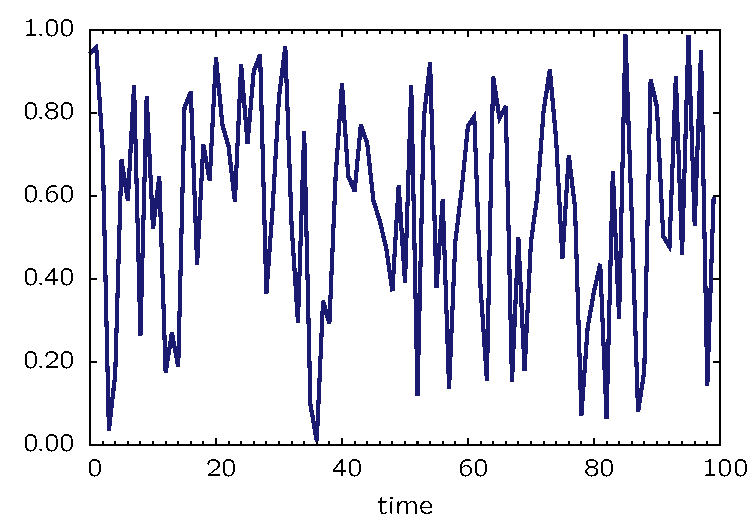
\includegraphics[width=0.75\textwidth]{rnum}
\end{center}

\foilhead[-1.5cm]{Checking}

How good are they? We should check: the marginal cumulative distribution (left), and
the apparent independence between consecutive values via the autocorrelation
function (right).

\begin{minipage}{0.48\textwidth}\centering
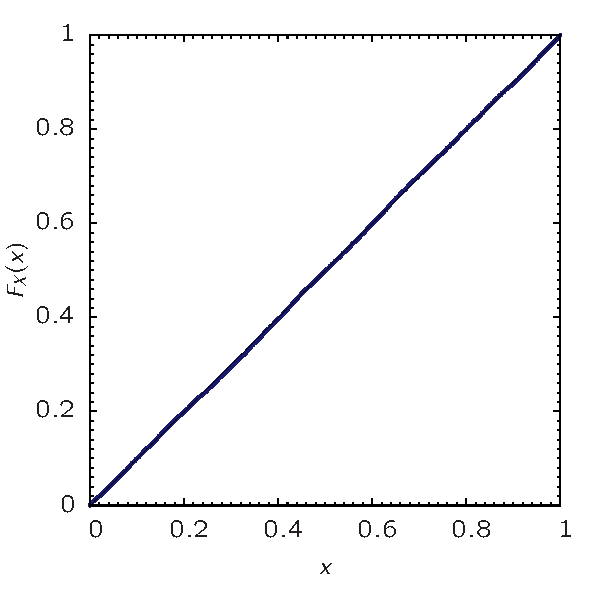
\includegraphics[width=0.8\textwidth]{rnum-cdf}
\end{minipage}
\hfill
\begin{minipage}{0.48\textwidth}\centering
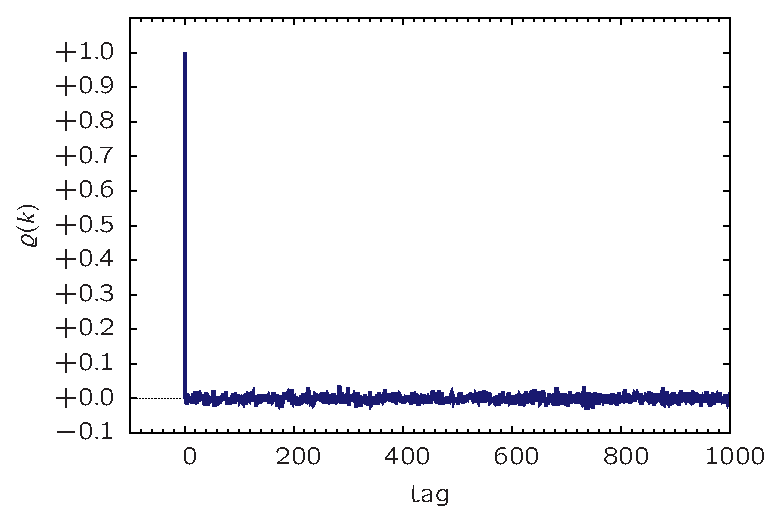
\includegraphics[width=\textwidth]{rnum-auto}\end{minipage}\pause

The 10000 pseudorandom numbers will look like 10000 independent realizations of
$X \sim U[0,1]$. \hl{But they were generated deterministically!}

\foilhead[-1.5cm]{Averaging physical equations}
We are all very used to Reynolds' decomposition and averaging equations, and treating the fluctuations as random variables:
\begin{align*}
\parder{\Theta}{t} &= - \parder{(U_k\Theta)}{x_k} + \nu_\theta\parpar{\Theta}{x_k}{x_k},\\
\Theta &= \tavg{\Theta} + \theta, \qquad U_k = \tavg{U_k} + u_k,\\
       &\vdotswithin{=} \\
\parder{\theta}{t} &= - \parder{}{x_k}\left[ \tavg{U_k}\theta + u_k\tavg{\Theta} +  u_k\theta - \tavg{u_k\theta}\right] + \nu_\theta\parpar{\theta}{x_k}{x_k},\\
       &\vdotswithin{=} \\
\parder{\tavg{\theta \theta}}{t} &=
-\tavg{U_k}\parder{\tavg{\theta\theta}}{x_k} 
-2\tavg{u_k\theta}\parder{\tavg{\Theta}}{x_k}
-\parder{\tavg{u_k\theta\theta}}{x_k} 
-2\nu_\theta \tavg{\parder{\theta}{x_k}\parder{\theta}{x_k}}
\end{align*}\pause
But can we really do it?

\foilhead{Averaging ensembles}

The equation 
\begin{equation*}
f(x) = (16807\, x) \bmod (2^{31} - 1).  \label{eq:rnum}
\end{equation*}
is a simple example of a \emph{dynamical system}. At the end of the 19th
century, physicists --- and engineers! --- were taking liberties and mixing
deterministic and stochastic approaches. A very nice review is given in
J. L. Lebowitz and O. Penrose, ``Modern Ergodic Theory'', \textit{Physics Today}
26(2), 26--29, 1973, from which we quote extensively:
\begin{quote}\small
The founding fathers of statistical mechanics, Boltzmann, Maxwell, Gibbs and
Einstein, invented the concept of ensembles to describe equilibrium and
nonequilibrium macroscopic systems.  In trying to justify the use of ensembles,
and to determine whether the ensembles evolved from nonequilibrium to
equilibrium, they introduced further concepts such as ``ergodicity'' and
``coarse graining''. The use of these concepts raised mathematical problems that
they could not solve, \hl{but like the good physicists they were they assumed that
everything was or could be made all right mathematically and went on with the physics.}
\end{quote}

\foilhead{Even so!}


(maybe I am a bad physicist or engineer :-))

I would like a little justification for mixing the deterministic and stochastic
approaches.


\foilhead{A brief chronology}

\begin{description}
\item[1871] Boltzmann introduces the ergodic hypothesis.
\item[1867] \cite{maxwell--dynamical.theory.gases} averages equations of motion for gas molecules.
\item[1895] Clearly influenced by Maxwell's paper --- but without mentioning
  Maxwell's name! --- Reynolds introduces his decomposition, $u = \overline{u} + u'$,
  which we still use today; he tries to found his equations on \emph{statistical
    mechanics}, and explicitly mentions at the introduction
  \citep{reynolds--b-dynamical} the ``kinetic theory of matter''. Reynolds
  derives the mean equations, and the equation for turbulence kinetic energy, by
  averaging essentially in the same way as we did for $\tavg{\theta\theta}$ in
  the introduction! However, ensemble averaging is not explicit; instead there
  is a mix of space and time averages.
\end{description}

\foilhead[-1.5cm]{(continued)}

\begin{description}
\item[1905] Einstein's \citeyear{einstein--uber.molekularkinetischen} theory of
  Brownian motion. Averaging equations of motion is not very explicit, but
  deterministic and probabilistic ideas are freely mixed \cite[see][]{einstein--movement}.
\item[1908] Langevin's \citeyear{langevin--brownien} paper on Brownian
  motion. Equations of motion are explicitly averaged
  \cite[see][]{lemons.gythiel--langevin.brownian}.
\item[1921] Taylor's \citeyear{taylor--diffusion} turbulent diffusion theory.
\item[1927] Birkhoff's \citeyear{birkhoff-proof-ergodic} proof of the Ergodic
  Theorem.
\item[1933] Kolmogorov's \citeyear{kolmogorov--foundations} book on the
  ``Foundations of probability theory''.
\item[1963] Lorenz's \citeyear{lorenz--deterministic} seminal paper on Chaos Theory
  was given the provisional title ``\hl{Deterministic turbulence}''
  \citep{motter.campbell--chaos.at.fifty}.
\end{description}

\foilhead[-2cm]{Four Perspectives on Probability}


\begin{center}
\url{http://www.ma.utexas.edu/users/mks/statmistakes/probability.html}
\end{center}

{\normalsize
\begin{enumerate}\zerolistvertdimens
\item \textbf{Classical} (sometimes called ``A priori'' or ``Theoretical''):

If we have a situation (a "random process") in which there are $n$
equally likely outcomes, and the event $A$ consists of exactly $m$ of these
outcomes, we say that the probability of $A$ is $m/n$. 
\textbf{This is circular reasoning!}


\item \textbf{Empirical} (sometimes called ``A posteriori'' or ``Frequentist'') This idea
  is formalized to define the probability of the event A as $P(A)$ = the limit
  as n approaches infinity of $m/n$, where $n$ is the number of times the
  process (e.g., tossing the die) is performed, and $m$ is the number of times
  the outcome A happens.

\item \textbf{Subjective}

Subjective probability is an individual person's measure of belief that an event
will occur. 

\item \textbf{Axiomatic}

This is \cite{kolmogorov--foundations}'s book.

\end{enumerate}}


\foilhead{Kolmogorov's definitive Probability}

A probability triple, or probability space, is a triple $(\Omega, \mathscr{F},
P)$, where:
\begin{itemize}\zerolistvertdimens
\item $\Omega$ is any non-empty set;
\item $\mathscr{F}$ is a $\sigma$-field, a collection of subsets of $\Omega$
  obeying special conditions.
\item $P$ is a function from $\mathscr{F}$ to $[0,1]$: $\mathscr{F}$ is the set
  or the class of subsets of $\Omega$ that can be ``measured''.
\end{itemize}
Several probability axioms hold, including the usual
\begin{align*}
P\{\emptyset\} &=0, \\
P\{\Omega\}    &=1, \\
A_i \cap A_j = \emptyset \Rightarrow P\left\{\bigcup_{i=1}^{\infty} A_i\right\} &= \sum_{i=1}^\infty P\{A_i\} \qquad
\text{(countable additivity)}.
\end{align*}

\foilhead{Random variables}

A random variable is a function $X: \Omega \to \mathbb{R}$ such that
\[
\left\{ \omega \in \Omega \;\big|\; X(\omega) \le x \right\} \in \mathscr{F}.
\]
$X$ is a \emph{measurable} function.


\begin{center}
   \includegraphics[width=0.3\textwidth]{/home/nldias/work/graduacao/matap/aulas/Xlessthanx}
   
   {Graphical representation of the event $X(\omega) \le x$}
\end{center}

\foilhead{Integration}

With Kolmogorov's axiomatic approach, things quickly fall into place.
The distribution function of $X$ is
\[
F_X(x) \equiv P\left\{ \omega \;\big|\; X(\omega) \le x \right\};
\]
with different degrees of sophistication and difficulty, one can now calculate
moments, such as the \emph{expected value}
\[
\tavg{X} = \int_{\Omega} X(\omega)\,\md{P}(\omega).
\]
Even better, a \emph{change of variable} theorem \citep[][Theorem
  6.1.1]{rosenthal--first.look} allows to do the same ``without $\Omega$'': for
any measurable function $ g: \mathbb{R} \to \mathbb{R}$,
\[
\int_{\Omega} g(X(\omega))\,\md{P}(\omega) = \int_{\mathbb{R}} g(t)\md{F_X}(t).
\]

\foilhead[-1.5cm]{The ``sample bag''}

Learning all this is hard; it is often good enough to think about it as the
sample bag $\Omega$ from which we draw numbers, beads, of any other concrete
representation of $X(\omega)$. Here it is again:

\begin{center}
   \includegraphics[width=0.35\textwidth]{/home/nldias/work/graduacao/matap/aulas/Xlessthanx}
\end{center}

\hl{But Kolmogorov did not --- and neither anybody else ever since --- ever teach us
how to draw an $\omega$ from the bag!}

\foilhead{Here is how I drew an $\omega$ in my program:}

\begin{alltt}\small\fboxsep0pt
#!/usr/bin/python
from math import floor
deno = 2**31
denu = 2**31 - 1
\colorbox{yellow}{xo = 0.9439494030244930249}
no = int(xo * deno)
fou = open('rnum2.out','wt')
fou.write("%8.6f %8.6f\textbackslash{n}" % (float(0),xo) )
n = 10000
for i in range(1,n):
   nn = 16807*no 
   xn = float(nn)/deno
   fou.write("%8.4f %8.6f\textbackslash{n}" % (float(i),xn) )
   no = nn
fou.close()
\end{alltt}\pause

In other words, I drew it myself!  This is what we all call the ``seed'' of the
random number generator.


\foilhead{The stochastic process}

Kolmogorov would not stop. From
\cite{todorovic--introduction.stochastic.processes}:
\begin{quote}
A stochastic process is a family of random variables $X(t)$, $t \in T$, defined
on a \emph{common} probability space $(\Omega,\mathscr{F},P)$, $T \subset \mathbb{R}$
\end{quote}
That is:
\begin{align*}
X : \Omega \times T &\to \mathbb{R},\\
    (\omega,t) &\mapsto x = X(\omega,t)
\end{align*}

The really important point to be made is this:
\begin{quote}
Once $\omega$ is chosen, $X(t)$ is \hl{deterministic}: an ordinary function
like any other!
\end{quote}

\foilhead{A ``bag'' for stochastic processes, too}

\begin{center}
   \includegraphics[width=0.6\textwidth]{/home/nldias/work/graduacao/matap/aulas/procest}

   \colorbox{yellow}{A single $\omega$ for each $x(t)$!}
\end{center}

\foilhead{Reconciling divorcees}

Now the random number generator is beginning to look like a stochastic process!

We can almost ``see'' the trick: if the function $f(x) = (16807\, x) \bmod
(2^{31} - 1)$ is ``measurable'' in some sense, then a single $\omega$ may spawn
a multidimensional vector $\vet{X}(\omega)$, which we may call, \emph{perhaps at
  the same time}, a \emph{stochastic process} \textbf{and} a \emph{dynamical
  system}.

\foilhead{Theorems of statistical mechanics and ergodic theory}

Let us extend --- and change --- nomenclature a little bit.  Let us call
$\Omega$ the \emph{state space} (also!). Let
\[
\omega \equiv x_0 \in \Omega,
\]
with
\begin{align*}
\phi_t: \Omega &\to \Omega, \\
x_0            &\mapsto x(t) = \phi_t(x_0).
\end{align*}
Above, $t$ can be either discrete (``maps'') or continuous (``flows''). We have
\begin{align*}
\phi_{t+s} &= \phi_s \circ \phi_t.
\end{align*}

\foilhead{What a dynamical system is}


A definition of a dynamical system is now the triple $(\Omega, \mathscr{F}, P)$
together with $\phi_t$.

This definition is essentially identical at first sight to that of a stochastic
process, but we must look at the conditions on $\phi_t$ and $P$ for the identity
to hold.

\foilhead[-1cm]{Measures}

As we already know from Kolmogorov's axiomatic
probability approach, the measure (probability) of a set $A$ in $\Omega$ is
\[
P(A) = \int_{x \in A} \md{P}(x).
\]
Let us say that $\phi_t$ is, in some sense, a measurable funcion. Then, if $P$ is a
probability measure on $\Omega$, then $\phi_t$ induces a new probability measure
in $\Omega$, by means of:
\[
P(\phi_t(A)) \equiv P(A) \qquad (\text{forward}).
\]
This is often done the other way around:
\[
P(A) \equiv P\left(\phi_{-t}(A)\right) \qquad (\text{backward}).
\]
If the above holds for all measurable $A \in \Omega$, we say that $P$ is
invariant under $\phi_t$.

\foilhead{The c�up de gr�ce}

From:
\begin{center}
Dynamical Systems and Stochastic Processes

(P. Collet, 2010)

\url{http://escuelainvierno.cimfav.cl/documentos/pdf/NotesP_Collet.pdf}
\end{center}

\begin{quote}\small
{Given a probability measure $\mu$ (read $P$) on the phase space $\Omega$ and the time evolution map
$T$ (or a (semi)-flow) (read $\phi_t$), we are \textbf{exactly} in the setting of stochastic processes.}
\end{quote}
This is because, given the dynamical system $\phi_t$, and a measurable function
$g$ on $\Omega$, we can define a stochastic
process $X(t)$ by means of
\[
X(\omega,t) \equiv g \left(\phi_t(\omega)\right).
\]

\foilhead{Could it be any clearer?}

Yes!\pause

\cite{collet--dynsys.valparaiso}:
\begin{quote}\small
The fact which may look a little unusual for a Probabilist is that the proba-
bility is given on the initial condition, \textbf{and there is no randomness
  appearing in the time evolution} (my emphasis). However the points on the
phase space completely characterize the orbits, and we can think of $\mu$ (read $P$) as a
probability measure on the orbits, the time evolution being the shift.

\hl{In that sense, any stochastic process is a dynamical system (a not very useful
remark in practice).}
\end{quote}

\foilhead{Ergodicity, and Birkhoff's theorem}

\[
\lim_{T\to\infty} \frac{1}{T} \int_0^T g(\phi_t(x_0))\,\md{t} = L
\stackrel{\text{if ergodic}}{=} \int_\Omega
g(\omega)\,\md{\omega}
\]

Remark: $X(x_0,t) = g(\phi_t(x_0)) $ is a single realization of a stochastic process from
  the initial condition $x_0$. The rightmost expression is \hl{independent of
    $x_0$, and only then is the process ergodic}.

Moreover, \citep{lebowitz.penrose--modern.ergodic}:
\begin{quote}\small
Stated precisely, this means that a system is ergodic on $S$ (read $\Omega$) if
and only if \emph{all} regions $R$ of $S$ (read $\Omega$) left invariant by the
time evolution, $\phi_t(R) = R$ either have zero area or have an area equal to
the area of $S$ (read either have zero probability measure, or have $P(R) = 1$).
\end{quote}

\foilhead{Being more accurate,}

However, the equality $\phi_t(R) = R$ in \cite{lebowitz.penrose--modern.ergodic}'s statement is somewhat
\emph{imprecise}!
Given the \emph{symmetric difference} between two sets, 
\[
A \;\triangle\; B \equiv (A \cup B)  - ( A \cap B),
\]
then, in terms of probability measure, the corresponding statement is.
\[
P\left(A \;\triangle\; \phi_{-t}(A)\right) = 0 \Leftrightarrow P(A) = 0 \; \text{or}
\; P(A) = 1.
\]
My simple-minded interpretation: in an ergodic system, the map $\phi_t$ makes
any realization eventually wander over \hl{almost all} of $\Omega$ ($P(A)=1$),
or \hl{almost none} of it at all ($P(A)=0$).

%% \foilhead{A word of caution on the terminology}

%% \cite[p. 40]{collet--dynsys.valparaiso}:
%% \begin{quote}
%% Birkhoff's ergodic theorem does not prove ergodicity .
%% It may be a very useful tool in proving ergodicity but as such it does not
%% claim it. In particular it applies in non-ergodic cases. Birkhoff's ergodic applies
%% as soon as you have an invariant measure. You have to work more to decide
%% whether or not the measure is ergodic.
%% \end{quote}

%% (I want to remove this remark for the final version for Santa Maria)

\foilhead[-1.5cm]{Example: Reynolds' postulates}

can now be regarded as lemmas:
\begin{align*}
   U_i &= \tavg{U_i} + u_i; \qquad \tavg{U_i}(\vet{x},t) = \int_{\omega \in \Omega} U_i(\vet{x},t;\omega)\,dP(\omega).\\
   \tavg{u_i} &= \tavg{ U_i - \tavg{U_i}} = \int_{\omega \in \Omega}
	          \left( U_i(\vet{x},t;\omega) - \tavg{U_i}(\vet{x},t)
	      \right)\,\md{P}(\omega) \nonumber \\
	      &= \int_{\omega \in \Omega} U_i(\vet{x},t;\omega) \,\md{P}(\omega) -
                 \tavg{U_i}(\vet{x},t)\int_{\omega \in \Omega} \,\md{P}(\omega) = 0.\\
   \tavg{u_i \tavg{{U}_j}} &= \int_{\omega \in \Omega}
			        u_i(\vet{x},t;\omega)
			        \tavg{U_j}(\vet{x},t)\,\md{P}(\omega) \\
			       &= \tavg{U_j}(\vet{x},t) \int_{\omega \in \Omega}
			        u_i(\vet{x},t;\omega)\,\md{P}(\omega)  \\
			       &= \tavg{U_j}\tavg{u_i} = 0. 
\end{align*}



\foilhead[-1.5cm]{Example: a non-ergodic process}

The stochastic process
\[
X(\omega,t) = U(\omega)
\]
with $U$ uniformly distributed on $[0,1]$ is stationary, but it is not
ergodic. Indeed, for instance,
\[
\Exv\{ X(t) \} = \Exv\{ U \} = 1/2, \; \text{etc.}
\]
but
\[
\lim_{T\to\infty} \frac{1}{T}\int_0^T X(t)\,\md{t} = X(0) \ne 1/2 \; \text{in
  general.}
\]

\foilhead{Picture of this non-ergodic process}

3 realizations:

\begin{minipage}{0.49\textwidth}
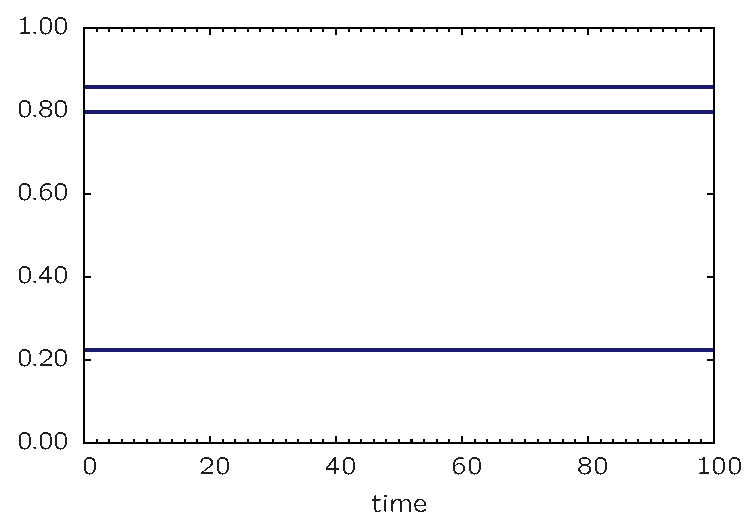
\includegraphics[width=\textwidth]{nonergodic}
\end{minipage}\hfill
\begin{minipage}{0.49\textwidth}
What is the problem?

This process has \emph{infinite} memory, and it does not wander all over $\Omega$.
\end{minipage}

\foilhead[-1.5cm]{The mixing condition}

implies (is a sufficient condition for) ergodicity:
\[
\lim_{\tau\to\infty} \int_\Omega f(x) g(\phi_{\tau}(x))\,\md{P}(x) = \int_\Omega f(x)\,\md{P}(x)
                                                                   \int_\Omega g(x)\,\md{P}(x)
\]
But
\[
C_{fg}(\tau) \equiv \tavg{f(x)g(\phi_\tau(x))} - \tavg{f(x)}\tavg{g(x)}
\]
is the $\tau$-covariance function; therefore,
\begin{quote}
If the $\tau$-covariance function goes go to zero, the process is ergodic.
\end{quote}
But this does not even guarantee that the process has finite variance.  For more
regularity, more conditions are needed.  \pause

The most common is the existence of
integral scales.

\foilhead[-1.5cm]{Ergodic, but nonstationary, and non-mixing}

The harmonic oscillator is
\begin{align*}
X(\omega,t)       &=  A(\omega)\cos t + B(\omega)\sen t, \\
\dot{X}(\omega,t) &= -A(\omega)\cos t + B(\omega)\cos t
\end{align*}
The state space is the circle
\[
\Omega: X^2 + \dot{X}^2 = R^2; \qquad X(\omega,0) = A(\omega), \; \dot{X}(\omega,0) = B(\omega).
\]
Without loss of generality, $R^2 = 1$.  We randomly pick a point $(A(\omega),B(\omega))$ on the
unit circle, and it will go round and round forever on it. The random point
actually corresponds to a uniform distribution of $\Theta(\omega) =
\arctgyx(B,A)$ on (say) $[-\pi,+\pi]$.

\foilhead{Numerical test of the harmonic oscillator}

$X(t)$ and $\dot{X}(t)$ wander all over $\Omega$, and the cdf of $\Theta$ is
recovered empirically: this is an indication that the process is \emph{ergodic}.
However, the autocorrelation function does not $\to 0$ as $\tau \to \infty$: the
process is non-mixing. Moreover, it is not stationary.

\begin{minipage}{0.48\textwidth}\centering
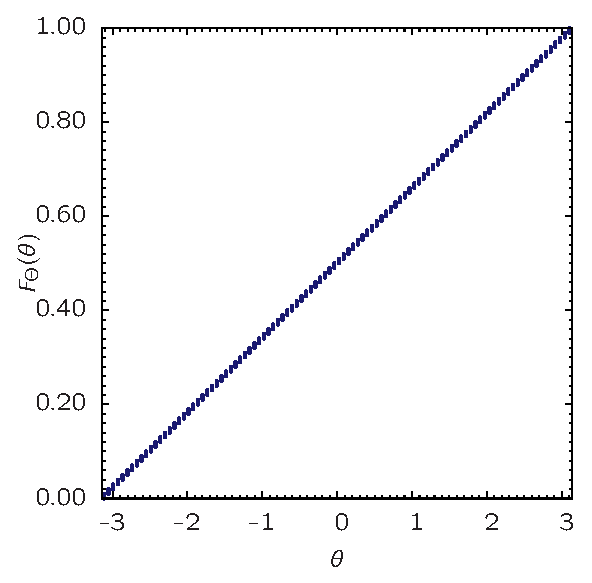
\includegraphics[width=0.8\textwidth]{harm-cdf}
\end{minipage}
\hfill
\begin{minipage}{0.48\textwidth}\centering
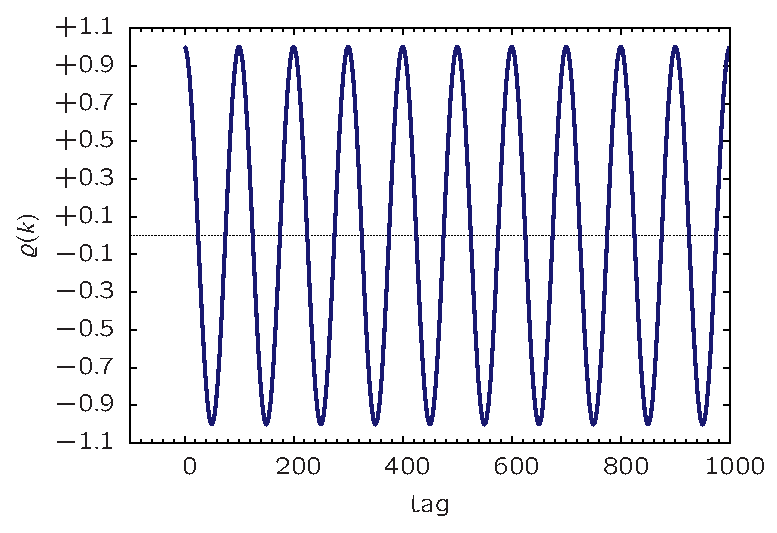
\includegraphics[width=\textwidth]{harm-auto}\end{minipage}



\foilhead[-1.5cm]{Example: the AR-1 process}

A multivariate random variable is a stochastic process. An n-uple
$(U_1, U_2, \ldots, U_n, \ldots )$
of zero-mean (without loss of generality), independent and identically
distributed random variables with variance $\sigma^2$ is a stochastic process,
if we look at it as:
\[
\mathbf{U}(\omega) = (U_1(\omega), U_2(\omega), \ldots, U_n(\omega), \ldots).
\]
Then this process can be used to build another one.  For instance, an
autoregressive, order 1 process
\begin{align*}
X_1 &= U_1\\
X_{n+1} &= \rho X_n + \sqrt{1 - \rho^2}U_{n+1}
\end{align*}
can now be seen as
\[
\mathbf{X}(\omega,n) = (X_1(\omega), X_2(\omega), \ldots, X_n(\omega), \ldots).
\]

\foilhead[-1cm]{Interpretation}

This is contrary to the usual first impression that in such a process there is a
``deterministic'' component ($\rho X_n$) and randomness introduced at each time
step ($\sqrt{1 - \rho^2}U_{n+1}$): we can alternatively think of all the
``randomness'' being drawn from the bag ``instantaneously'' ($\mathbf{U}(\omega)$) and
a deterministic function $X(\omega,n)$ being defined once $\omega$ has been
drawn.

%% We then have
%% \begin{align*}
%% \Exv\{ X_{n+1} \} &= \rho \Exv\{ X_n \} = \ldots = \rho \Exv\{X_1\} = 0, \\
%% \Var\{ X_{n+1} \} &= \rho^2\Var\{ X_n \} + (1 - \rho^2)\Var\{ U_{n+1}\} = \sigma^2.
%% \end{align*}

\foilhead{So, what is ``random''?}

\pause
I don't know.
\pause

\begin{itemize}\zerolistvertdimens
\item Kolmogorov axiomatized it: ``there exists'' a probability measure, with highly
sophisticated mathematical aspects.
\item He didn't teach us how to ``draw''.
\item We remain dependent on \hl{analog sampling devices} when it comes to
  ``drawing'': we use bit traffic over the internet, repeated laboratory or
  field experiments, or good old dice and roulettes.
\end{itemize}

In short: \hl{I think} we do not know what ``random'' is.  Perhaps it is just another label
for an ``unpredictable'' process.\pause

(Even if it is deterministic, and (in the sense of the gods), pre-ordained.)

\foilhead[-1.5cm]{Conclusions}

\begin{itemize}
\item ``Ergodic'', ``Stationary'' and ``Mixing'' do not always flock together.
\item To a large extent, stochastic processes and dynamical systems can be given
  a unified treatment. There are technicalities, like the nature of the
  measures, and the sigma-fields involved, etc.. 
\item At any rate, this unified approach justifies the liberties taken for
  instance in averaging turbulent flows both analytically and in the
  laboratory/field. 
\item A long way lies ahead, however.  For instance: are the Navier-Stokes
  equations ergodic? How about mixing?
\item Reynolds' approach in averaging the Navier-Stokes equations antedates
  important and seminal work on Statistical Mechanics and Ergodic Theory. It
  remains far-reaching and an important tool to this day.
\end{itemize}


\foilhead{That's it}

\vfill

Thank you very much for the attention.

\vfill

\foilhead{References}



\bibliography{all}
\bibliographystyle{aaai-named}


\end{document}




